\chapter{\texttt{srg1d} Python Library}\label{python_lib}

In this chapter, we discuss the design and features of the \texttt{srg1d} Python library. The development of this library was a significant portion of the work that led to this thesis. We will begin by discussing the practical importance of a careful, conscious approach to programming for physics, followed by a review of some programming concepts and terms to facilitate the explanation of the library. We will also speak briefly about the Python programming language and the reasons it was chosen for this project. Then, we will move into the design of the library overall as well as the specific parts. Finally, we will discuss details regarding the implementation and testing the library.

\section{Philosophy of Programming for Physics}

The three principles that guided the programming done for this work are modularization, validation, and abstraction. By writing modular code, we isolate logically independent portions of our project that offer some functionality that is useful on its own. These independent parts can then be applied only to those problems to which they are useful. We can also validate the implementation of these isolated functions, testing them through unit tests or by comparing their results to the results of other implementations. Unit tests are especially useful because they isolate specific use-cases. When changes are made to the codebase, running a comprehensive suite of unit tests can give developers a good idea of what features these changes affected and where they can go to fix the new bugs. Finally, with properly modular code, it is possible to offer logical abstractions that allow the user to avoid thinking about low-level implementation details and work in terms of objects that are relevant to the problem at hand.

These principles are realized by most software engineering projects, where maintainability and collaboration are central concerns. However, we feel that they are equally valuable when developing codebases for physics research, for the same reasons. Projects that follow these principles will allow for easier collaboration and set a solid foundation for projects that are extensions of the current work, in addition to bug detection and identification benefits of the approach.

\section{Review of Programming Concepts}

This review assumes the reader has a basic understanding of programming and aims to explain certain programming concepts and communicate their practical importance. This will better equip readers to understand the rest of the chapter.

\begin{itemize}
    \item \textbf{Classes} are a way for programmers to create complex objects for cases where the programming language basic types (integers, floating point numbers, strings, booleans, arrays) are not enough to meet their needs. A class has some internal data, as well as methods and properties which interact with that internal data. A user can create an object of a class by calling its constructor method. It can interact with the object through its interface.
    \item \textbf{Interfaces} define how a user can interact with an object, through methods and properties. Methods typically change the object in some way or do some significant evaluation of the object internals. Properties allow users to extract certain properties of the object, without changing them.
    \item \textbf{Collections} are classes that contain a bunch of similar objects and define how users can access the objects in the collection. Different variations of collections exist to enforce some conditions on the collection, such as no duplicates or limited ways to access objects in the collection.
    \item \textbf{Indexing} is an operation defined on a collection which allows a user to get any object in the collection by providing the collection the proper index. The simplest example of indexing is a standard array, which most people who have used a programming language have seen.
    \item \textbf{Iterating} on a collection is a way for a user to sequentially access every object in a collection. For a user, accessing objects in a collection via iteration requires the user to know as little as possible about the collection or how to actually access the objects in the collection. Some collections guarantee that the order of the objects accessed via iteration is the same every time as long as the collection is not modified. 
    \item \textbf{Mutability} is the ability of an object to be modified by the user after it is created. Mutable objects (or objects that can change by something the user does) give the user more flexibility in terms of possible functionality, but open the door for potential misuse by the user when properties of the collection are saved by the user, the collection is modified, and those saved properties are not updated to reflect the changes. Immutable objects make sense in cases where the objects should not change, like an array of the days of the week.
    \item \textbf{References} allow multiple objects to have access to the same thing. If the reference to an object is given to two different objects and the first modifies the referenced object, the changes will be reflected in the second object as well. This can lead to difficult-to-manage behavior. As a result, it is good to use references in conjunction with immutable objects, because, in that case, both objects can be sure that the object their reference refers to will never change.
\end{itemize}


\section{A Note on the Python Programming Language}

Python is a dynamically-typed, interpreted, high-level programming language that is used for general-purpose programming. Python is used by many, both inside and outside the sciences, and according to StackOverflow, it has ``a solid claim to being the fastest growing major programming language." Python currently has two supported major versions, Python 2 and Python 3, with Python 2 being supported for developers unable to immediately transition to Python 3.

Although the numerical libraries in Python are quite fast due to their low-level C bindings, Python is still not a high-performance language. Projects written in Python that are not satisfied with their performance can profile their code to identify bottlenecks and take advantage of Python bindings to low-level languages like C and Fortran to speed up work-intensive portions of their program. The Pareto principle applied to programming states that 80\% of the work of a program will be done by 20\% of the code, which we call the work-intensive part of the code. A profiling tool like \texttt{cProfile} can be used to help the developer identify these portions. Python's C implementation, Cython, has native C bindings that allow developers to call C subroutines, which will allow them to achieve their desired performance.

However, despite the general computational challenge faced by nuclear theory in general, the simple 1-dimensional system explored here is numerically relatively simple. Thus, high throughput and efficient memory usage are not requirements for these calculations to be done in a reasonable amount of time on any modern personal computer. In addition, Python is extremely expressive with a large standard library and well-documented third party libraries, making developer productivity very high. This was a priority in this research, leading to the decision to work in Python.

The next section discusses the general design of the library and references the interfaces for various different classes. A feature of Python is that users with sufficient knowledge of the internal representation of data in Python classes can directly access those internals and use or modify them how they see fit. This means that published interfaces don't truly limit what a user can do with a library and things like immutability are difficult or impossible to truly enforce. However, Python developers have the philosophy that all Python users are ``consenting adults." This means that the documentation of interfaces and conditions on the objects like immutability are communicated to users in an understanding that they should stick to these documented designs if they expect things to work as advertised.

\section{Library Design}

The class-based abstractions offered by the library offer consistent representations of different logical classes of objects present in any SRG calculation. By offering the user classes and functions that handle much of the complex, but frequently required functionality in any SRG calculation, the library allows the user to focus on exploration and research rather than reinventing the wheel. Behind the abstractions in the library are also several checks that ensure the physical correctness and consistency of what the user is doing. This further boosts user productivity, as the library provide transparent clear errors as to what conditions were not met, allowing the user to quickly understand where the error in their program is.

\begin{figure}[t]
\begin{center}
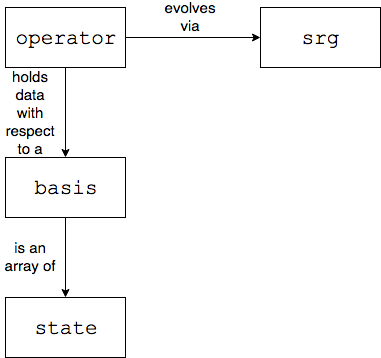
\includegraphics[width=0.6\linewidth]{srg1d}
\end{center}
\caption{A general structure for the modules in the \texttt{srg1d} library.}
\label{fig:srg1d}
\end{figure}

The library is roughly split into two logical halves. The data representation half (\texttt{state}, \texttt{basis}, and \texttt{operator}) handles the representations of the matrices for the operators in the calculations. Its primary goal is to add the context to the numerical representation of matrices and as a result make transformations of those matrices easier to achieve. The evolution half of the library (\texttt{srg}) handles the SRG transformation of the data. While the data representation classes correspond to concrete objects, the \texttt{srg} class is more of a state machine that allows the user to put some data in, turn the crank, and get out intermediate and final results.

\subsection{\texttt{state}}

The \texttt{state} module provides the fundamental building blocks for the data representation side of the library. It contains two classes, \texttt{ho\_state\_2body} and \texttt{ho\_state\_nbody}, that implement the same simple interface. The interface for both classes simply defines a constructor and \texttt{val}, a method to evaluate the harmonic oscillator wavefunction that the state corresponds to at some momentum. These classes are intended to add context data (harmonic oscillator number, number of particles, dirac notation) to the wavefunction that will simplify the evaluation of the wavefunction and allow for the construction of states with more complex structures due to additional physical conditions imposed on the states, like symmetry. Because these states are only intended to be used to get wavefunction values, their interface defines them to be immutable.

\texttt{ho\_state\_2body} represents a 2-body harmonic oscillator state. \texttt{ho\_state\_nbody} is different from \texttt{ho\_state\_2body} in that it represents a general linear combination of $n$-body product states. The only conditions on this linear combination of product states are that it is normalized and that the total harmonic oscillator number for each product state in the linear combination is the same. \texttt{ho\_state\_2body} is the basic building block of these general $n$-body product states.

It is worth mentioning that \texttt{ho\_state\_nbody} does not enforce any symmetry on these states. The conditions imposed on the linear combination of product states are the minimum conditions for such a state to be physically useful. The burden of ensuring proper symmetry falls on the operations creating the states, which is handled elsewhere in the \texttt{srg1d} library. Thus, for the purposes of an SRG calculation, a user should never have to deal with the \texttt{state} module directly.

\subsection{\texttt{basis}}

The \texttt{basis} module provides a basic interface for a \texttt{basis} class and two classes, \texttt{p\_basis} and \texttt{ho\_basis}, that implement this interface. The \texttt{basis} class interface comprises only a constructor, but it also defines \texttt{\_\_len\_\_}, giving the size of the basis, and \texttt{\_\_getitem\_\_}, allowing the user to access a state by its index. These additionally defined methods make any basis indexable and iterable, with iterability being especially valuable for working with bases. The classes that implement the \texttt{basis} interface are also defined to be immutable, because after construction these bases have certain properties (symmetry, completeness, etc.) that would be disturbed by the removal, addition, or modification of a state in the basis.

\texttt{p\_basis} is the representation of a momentum basis. Strictly speaking, a momentum basis is a continuous basis, that is operators need to be defined for any pair of real momenta. However, for numerical purposes, it makes sense to discretize the momentum space and impose some upper and lower cutoffs on momenta included in the basis. The upper and lower cutoffs on a discretized momentum basis are left to the user, who can judge what the range of relevant momenta is. The discretization scheme for the points between those upper and lower bounds is given by a Gaussian quadrature, which provides points $p_i$ and weights $w_i$ at which to evaluate the function. This provides us with the momentum basis for a single Jacobi momentum. From the single momentum basis, we can generate the two Jacobi momentum basis by taking the Cartesian product between two single momentum bases, with the weight assigned to to each new state being the product of the two weights corresponding to the states in the ordered pair. This approach can be used to generate a basis for any number of Jacobi momenta. The data representation of the $n$-body momentum basis is simply a list of these states, which are represented as $n$-tuples with $n-1$ Jacobi coordinates and finally a weight for the state.

\texttt{ho\_basis} is the representation of a harmonic oscillator basis. This is simply a list of harmonic oscillator states (2-body or $n$-body) up to some maximum total harmonic oscillator number, $N_{max}$. The standard constructor for \texttt{ho\_basis} generates a basis of 2-body states with proper symmetry. \texttt{ho\_basis} has a second constructor \texttt{ho\_basis.from\_basis} that takes any $n$-body \texttt{ho\_basis} object and generates an appropriately symmetrized $n+1$-body basis. Additionally, each $n$-body basis has a reference to the $n-1$-body basis used to generate it, which is useful for functions which need to recurse down to the 2-body basis. Because generating bases with appropriate symmetry is an expensive operation, it is important to avoid recreating \texttt{ho\_basis} objects. Thus, the \texttt{srg1d} library makes an effort to work with references to existing objects whenever it is possible.

\subsection{\texttt{operator}}

The \texttt{operator} module provides a simple \texttt{operator} class which couples a matrix with a basis that corresponds to its representation along with several additional useful methods that work on operators. The packaging of a matrix and a basis into one object reduces the potential for bugs when calling methods that require both the data and the basis, which occurs frequently in the setup of an SRG calculation. It also ensures that methods requiring operators can be certain that the basis and matrix are consistent, so methods do not need to do redundant checks, such as ensuring the basis and data sizes match.

The methods provided by the \texttt{operator} module do one of three things: generate operators, transform operators, or embed operators. The operator generating methods, \texttt{create\_ho\_basis\_kinetic\_energy}, \texttt{create\_p\_basis\_kinetic\_energy}, and \texttt{create\_kinetic\_energy}, are methods that calculate the kinetic energy operator in a certain basis and return a corresponding \texttt{operator} object. While the general $n$-body kinetic energy can be calculated directly, the $n$-body kinetic energy is calculated recursively, with the 2-body kinetic energy being the base case. This is where the $n$-body \texttt{ho\_basis} internal reference to the $n-1$-body \texttt{ho\_basis} comes in handy.

The \texttt{transform\_operator\_to\_p\_basis}, \texttt{transform\_operator\_to\_ho\_basis}, and \texttt{transform\_operator} methods all compute a unitary transformation for the operator data between a harmonic oscillator basis representation and a momentum basis representation. The harmonic oscillator basis has a parameter $\omega$ which relates to the strength of the oscillator; this value needs to be optimized for the transformation from momentum space to harmonic oscillator space. If no value is given for $\omega$ in the function call, it will be optimized internally and return with the transformed operator. A transformation from harmonic oscillator space to momentum space requires the $\omega$ used originally to transform the operator to harmonic oscillator to be passed in by the user. A future implementation may add an internal member to the \texttt{operator} class keeping track of $\omega$ for operators in harmonic oscillator space to avoid placing the burden of keeping track of the value on the user.

Finally, \texttt{embed\_operator} embeds an operator in harmonic oscillator space in a higher-body harmonic oscillator basis provided by the user. The logic for this embedding is similar to the logic for generating the general $n$-body kinetic energy in harmonic oscillator space. Again, this algorithm takes advantage of the internal reference to the $n-1$-body basis kept by the $n$-body \texttt{ho\_basis} to avoid recreating a new equivalent basis.

\subsection{\texttt{srg}}

The \texttt{srg} module only contains the \texttt{srg} class, which handles the evolution of some operator via the SRG flow equation. The three methods of this class are its constructor, \texttt{evolve}, and \texttt{set\_generator}. The constructor takes in a potential and a kinetic energy (which are the Hamiltonian when added up), as well as a 2-tuple of matrices called the generator. These two generator matrices are weights assigned to matrix elements of the potential and kinetic energies that are used when computing the flow operator $G_s$. For the standard $G_s = T_{rel}$, a zero matrix for the generator corresponding to the potential energy and a matrix of ones for the generator corresponding to the kinetic energy is one way to compute the correct flow operator. Allowing the user to provide a function to compute the flow operator from the kinetic and potential energy was a design that was considered, but rejected in favor of the easier-to-check and less complex generator matrices. The \texttt{set\_generator} method allows the user to alter the flow operator used between evolutions. While it is not typically useful to change flow operators part of the way through a full SRG calculation, this was added to allow us to easily switch between operators during calculations and investigate how composite SRG evolutions affect results.

The \texttt{evolve} method evolves the Hamiltonian provided in the constructor to a specified value of the flow parameter $\lambda$. The method uses \texttt{scipy.integrate.ode} to solve the system of coupled differential equations. In addition to taking the target value of $\lambda$ as a parameter, it also optionally takes parameters to specify an integrator and parameters for that integrator for users with specific needs who are also familiar with the integrators available through the \texttt{scipy.integrate.ode} method. The default integrator used is \texttt{\'dopri5\'}, a fourth order Runge-Kutta method that works well for non-stiff systems. However, for problems that are more stiff, it makes sense to switch to \texttt{\'lsoda\'}, a solver that dynamically switches between different algorithms for non-stiff and stiff problems. The only downside to the \texttt{\'lsoda\'} integrator is that it is not re-entrant meaning that different \texttt{srg} objects cannot both use it at the same time and therefore would be unable to run in parallel. The \texttt{srg} class also has accessor functions to allow the user to quickly access the data of the evolved potential as well as the current value of the flow parameter $lambda$.

\section{Implementation}

The first version of the library was written to be compatible only with Python 2.7. We made a decision fairly early on to focus development on Python 3, with an auxiliary goal of still being Python 2 compatible. Over time, the attention paid to keeping the code Python 2 compatible waned. As a result, it is currently not able to be used in Python 2. Fortunately, the recent Python Developers Survey 2017 published by Jetbrains shows that Python 3 is used by 75\% of Python developers as their primary version of the language, a substantial shift from 2013, when this project began, and 2015, when the switch to Python 3 on the project was made. Additionally, Python 2 will officially stop being supported in 2020. All of this leaves the \texttt{srg1d} library in a good place considering Python 3 adoption trends and the waning support for Python 2.

\subsection{Libraries Used}

The only non-standard libraries used in \texttt{srg1d} are NumPy and SciPy. NumPy arrays are convenient for representing vectors and matrices and can be used interchangeably with lists and lists of lists. Additionally, they allow for efficient numerical calculations and are the standard representation for data throughout the NumPy and SciPy libraries. NumPy also offers matrix and vector operations. SciPy extends the utility of NumPy by offering more linear algebra functions such as eigenvalue decomposition and numerical solvers for systems of coupled differential equations. Both NumPy and SciPy are available in the Python Package Index (PyPI) and can be installed easily with the Python package management system, \texttt{pip}.

\subsection{Handling Unexpected Usage}

It was mentioned previously that Python relies on library implementers and library users being ``consenting adults." As far as libraries are concerned, this means library implementers only have an obligation to document the interface, not actually enforce it. This is different from programming in languages like C++ or Java, where static typing forces users to adhere to an interface. In fact, Python users typically take the stance that if a library user is able to provide an object that doesn't strictly match the library interface but interacts with the library implementation in a way that works, that usage is fine. This is known as ``duck typing," following the principle ``if it walks like a duck and talks like a duck, then it must be a duck." In keeping in line with this philosophy, the \texttt{srg1d} library never enforces the type of objects using \texttt{isinstance}. Instead, it typically checks that an object implements the necessary interface, which is done by checking the existence of the required methods and properties.

However, in cases where data is taken in but not used, like in an object constructor call, it makes sense to ensure that errors that will definitely lead to problems later are immediately detected and pointed out to the user. Examples of this include checking that matrices that will be multiplied later have the correct dimensions and checking that corresponding bases and matrices have the same length. The implementation of the \texttt{srg1d} library strives to do comprehensive checks in this regard wherever it is reasonable, primarily in object constructors.

One notable exception to this rule is the \texttt{val} method from the \texttt{ho\_state\_2body} and \texttt{ho\_state\_nbody} class. This method is ideally never directly called by the user, but profiling done with \texttt{cProfile} showed that around 75\% of time spent initializing the SRG calculation (calculating operators and transforming or embedding them) was spent inside of it. Removing the checks done on the parameters in \texttt{val} halved the time spent inside it. Outer loop optimizations also reduced the number of calls to the method from several million to several hundred thousand. As the library is designed to make it so the user never has to use this method and it is so frequently called, we believe removing error checking from it is worth the performance. In cases where the user does need to directly work with the \texttt{ho\_state\_2body} and \texttt{ho\_state\_nbody} objects, they still have the documentation of the interface to fall back on.

\section{Testing}

An effort was made to adopt a test-driven development (TDD) approach in the development of the \texttt{srg1d} library. Tests are written using the \texttt{unittest} standard Python library, and the documented way to run the tests involves using \texttt{nose}. \texttt{nose} is an extension to \texttt{unittest} that can easily be installed via \texttt{pip}. The installation of \texttt{nose} comes with a script called \texttt{nosetests}, which can be run by the user and will automatically discover and run tests. While the project does not have complete code coverage, the existing tests focus on object constructors and specifically on graceful failure when these constructors are incorrectly called. The \texttt{state} module has good test coverage of the \texttt{val} method for both classes. One of the goals for the library before publication of the package is to extend the current incomplete test suite to have better coverage.


